%&latex
%
\documentclass[../template.tex]{subfiles}
\begin{document}

\lesson{4}{20/3/20}

\section{M/G/1 Queue}
A more complex model for the queueing system is given by considering different service times for each customer, and treat arrivals as a \textbf{Poisson}  process. This leads to the \textbf{M/G/1 model}.

\begin{itemize}
    \item The first letter denotes the type of the interarrival distribution, which in this case is intended to be \q{Memoryless}, and thus \textbf{exponential}. 
    \item The second letter describes the distribution of the service time. $G$ stands for \q{general}, meaning that we don't make any assumption on that pdf.
    \item The $1$ at the end is the number of servers, i.e. the number of clients that can be served at once.
\end{itemize}

As in the previous case, a customer arriving when the server is free will go immediately to the service, while others will wait their turn in an orderly queue. If at any time there are no customers being served and no arrivals, no service will be given.

\medskip

We could be tempted to define $X(t)$ as the number of customers in the system at $t$, and then consider the stochastic process $\{X(t), t \geq 0\}$. Unfortunately, this is not a Markovian process, as it not satisfies the Markovian property. The amount time elapsed from the last arrival \textit{does not matter} for the distribution of arrival times (as it is memoryless). However, the departure times \textit{do} depend on past information. As we assume a \textit{generic} distribution for the service time, it won't necessarily be memoryless, meaning that the time until the next departure depends on how much time has passed from the service's start, which is information \textit{not contained} in just the state $X_t$. 

\begin{appr}
    Note that in the previous example we circumvented this problem by fixing a definite, deterministic, duration for the service: one customer is served in a single time slot. Here we are not making such assumption.
\end{appr}

To reduce the system to a Markov process, we can just include the necessary information (how much time the user currently being served has been there) in the current state. However, this will make the model much more complex.

\medskip

Another way is to \textit{discretize time}, by sampling $X_t$ just at the departures' time. This is a variation of the \q{time slots} we used in the first examples - however in this case the time slots are not all of the same size, and their duration is not deterministic. 

In fact, when a customer departs at instant $\bar{t}$, the behaviour of the system is fully specified by the $X_{\bar{t}}$ at that time. If $X_{\bar{t}} > 0$, then the next user in queue will be served, and if $X_{\bar{t}} = 0$, nothing happens.

\medskip

This is one example of a more general trick: often a process $\{X_t\}_{t \in \mathbb{R}^+}$ is not a Markov process, but a \q{discretized sample} $\{X_{t_i}\}_{i\in \mathbb{N}}$ for a certain \q{good} choice of instants $\{t_i\}$ is a Markov process.

\begin{figure}[htp]
    \centering
    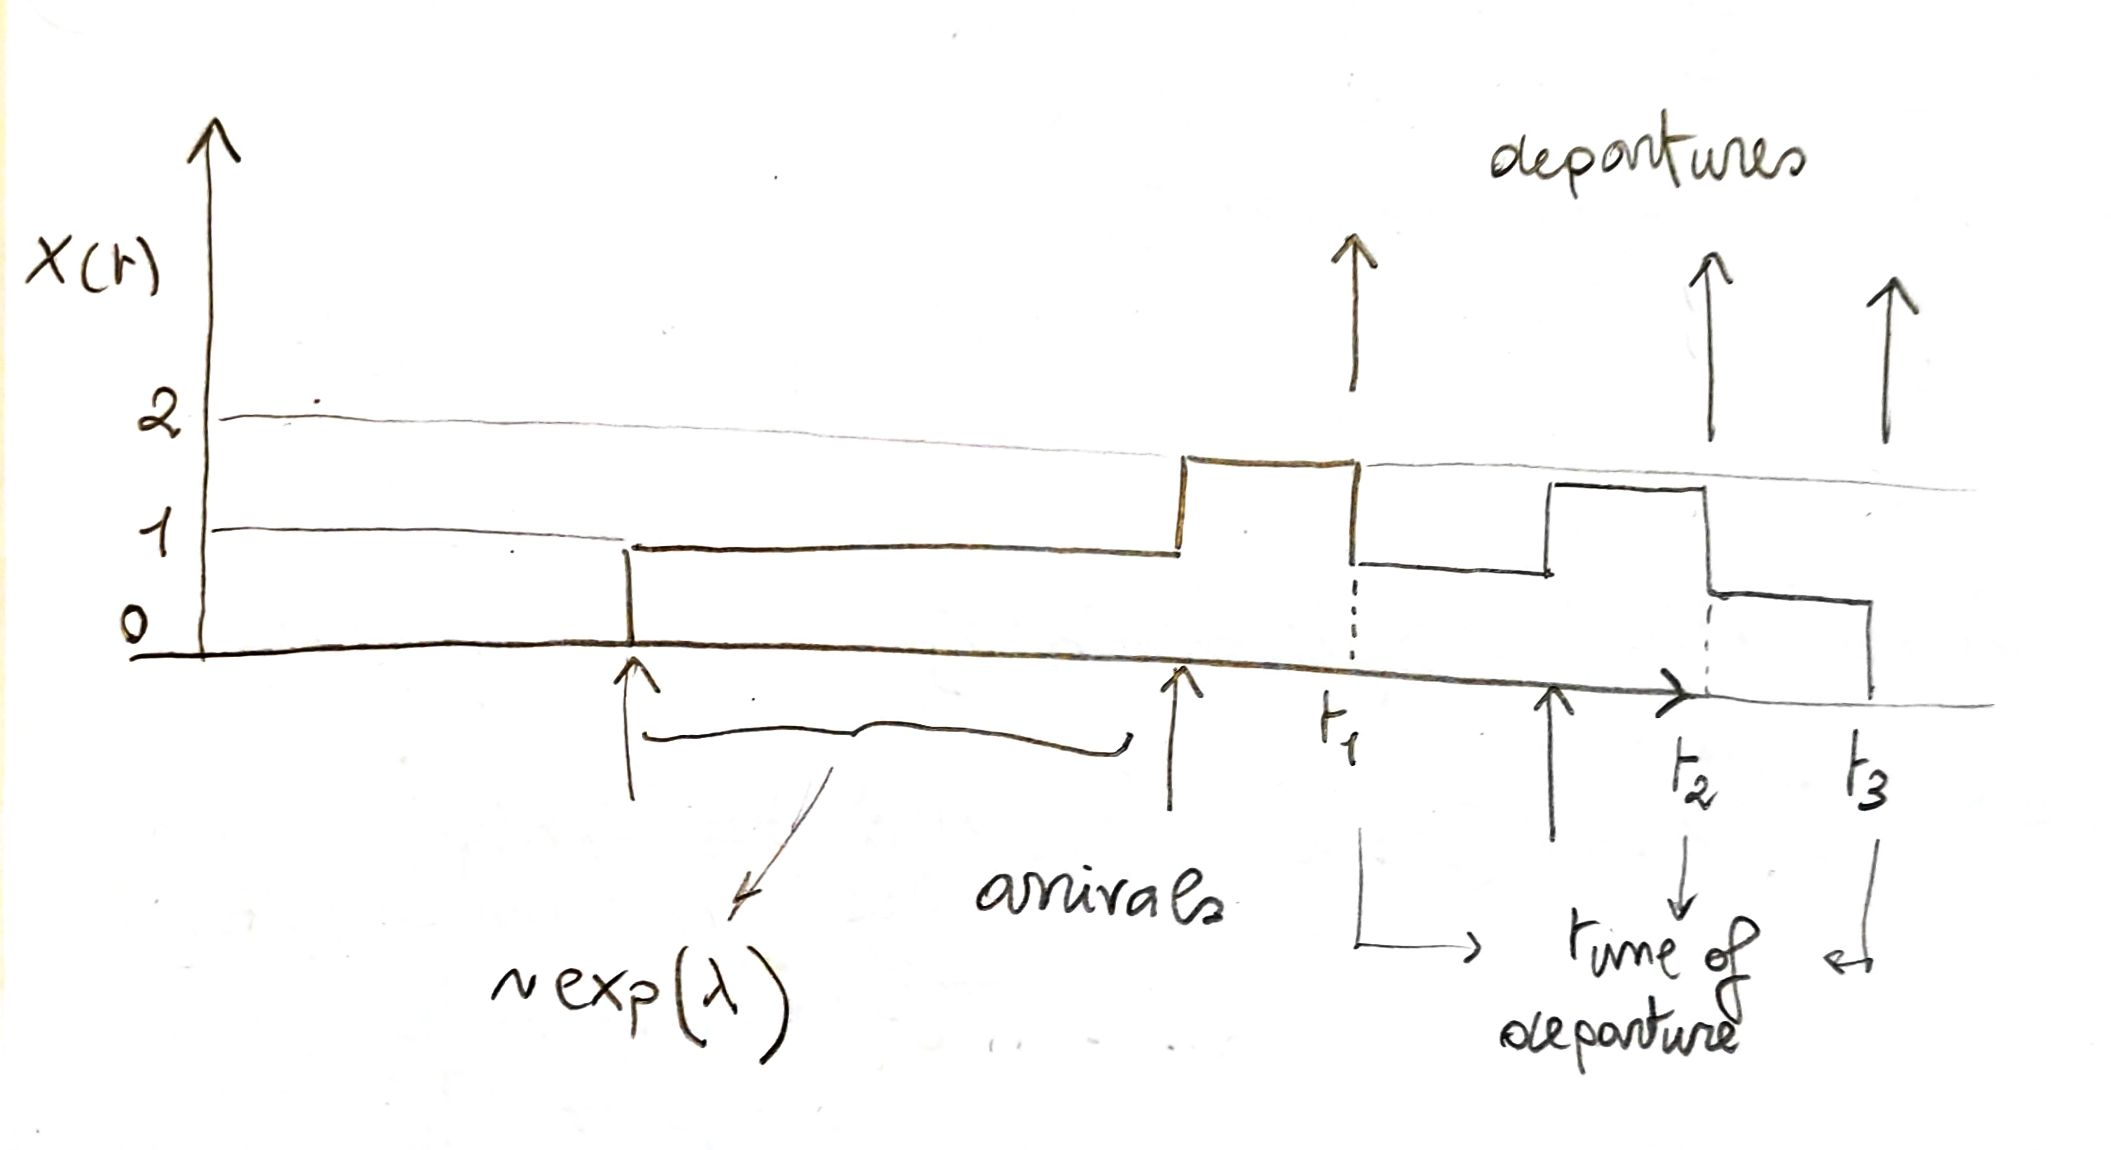
\includegraphics[width=0.7\textwidth]{MG1-graph1.jpeg}
    \caption{Example of evolution for the MG1 queuing system\label{fig:queue-ev1}} 
\end{figure}

So, let's denote with $t_n$ the time of the $n$-th departure, and with $X_n \equiv X(t_n^+)$ ($n \geq 1$) the number of customers in the system \textit{left behind} by the $n$-th departure\footnote{In a sense, we are inspecting $X_t$ \textit{slightly after} $t_n$, i.e. at $t_n^+$, which is just after the $n$-th departure, but before any new arrival.}, as illustrated in fig. \ref{fig:queue-ev1}.

\medskip

We also denote with $Y_n$ ($n \geq 0$) the number of arrivals occurring during the service time for the $n$-th customer, which is given by the difference between $t_n$ and the arrival time of that customer. If the queue size is $>0$, then the latter will simply be $t_{n-1}$, as illustrated in fig. \ref{fig:queue-ev2}.

\begin{figure}[htp]
    \centering
    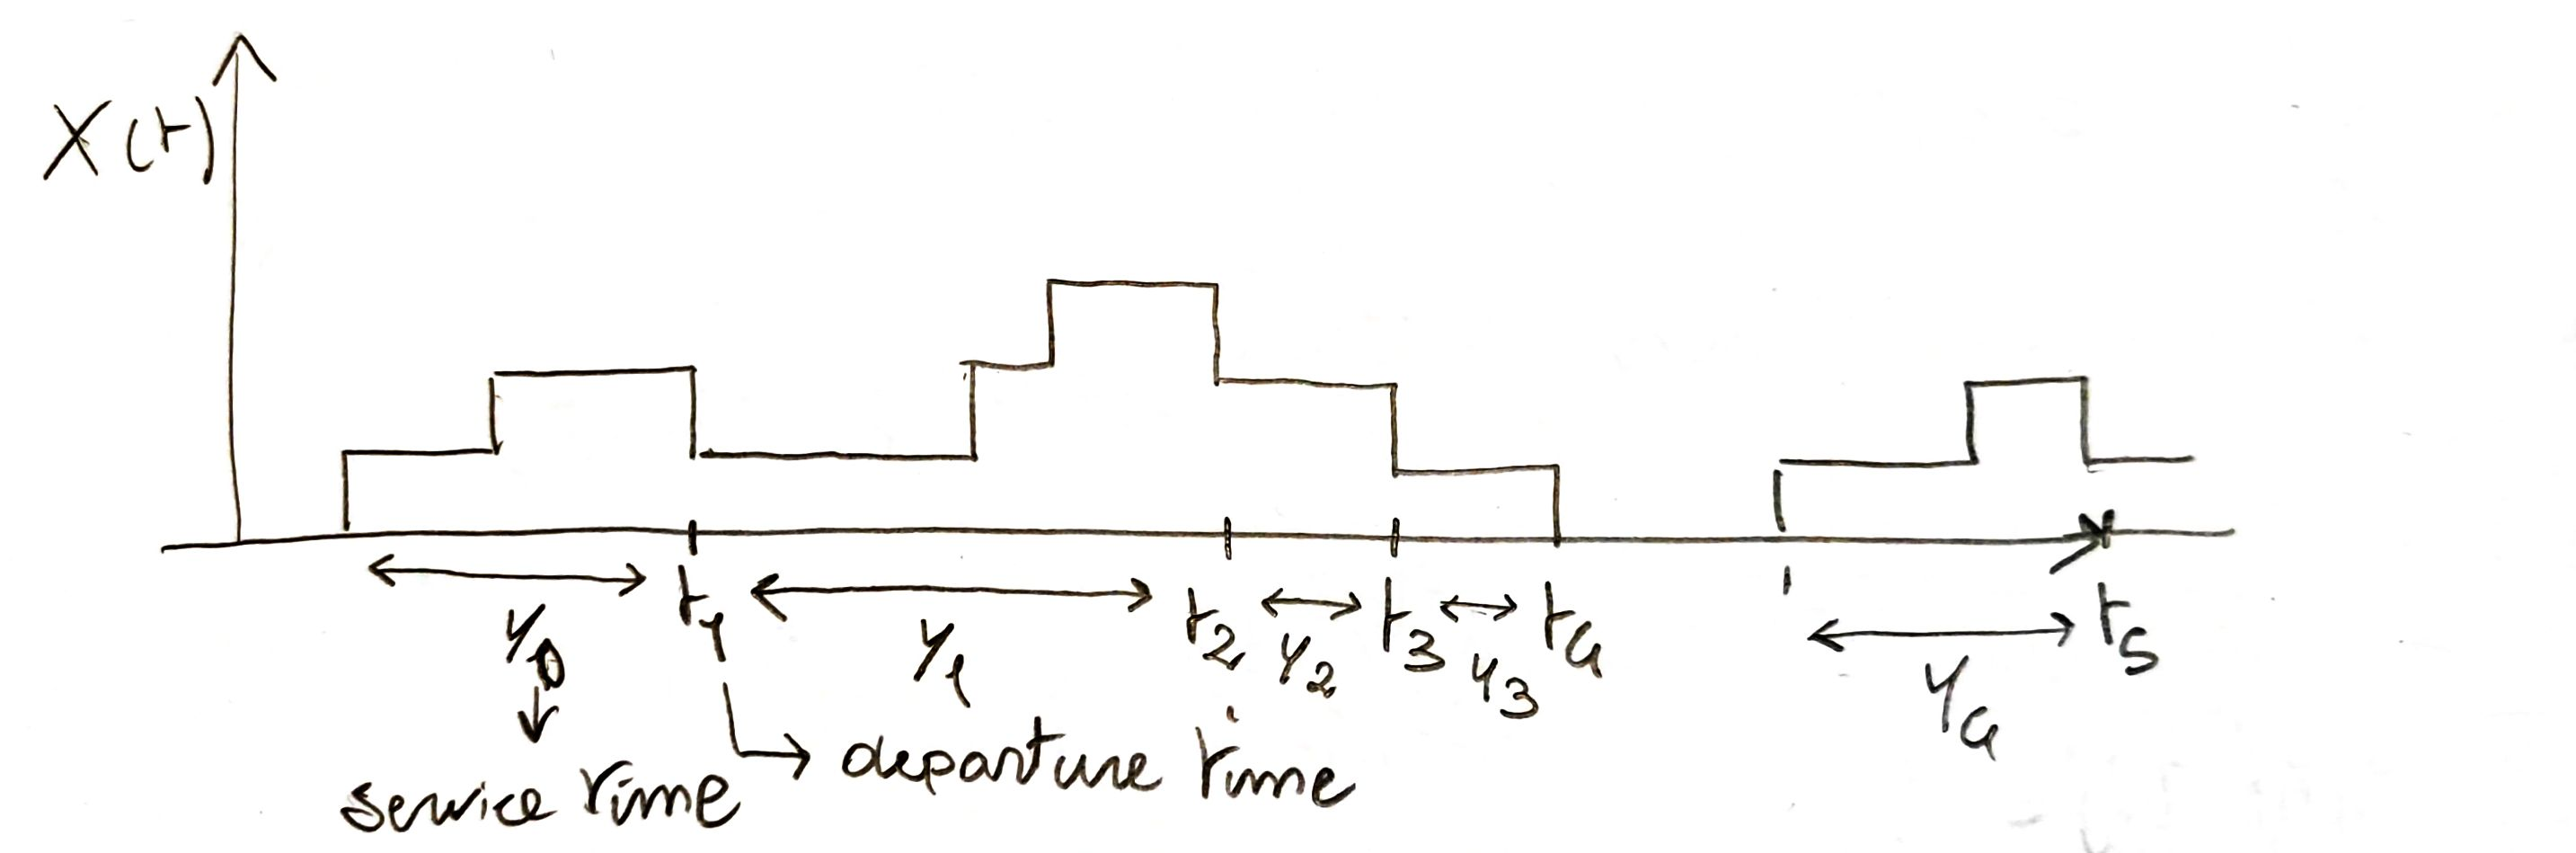
\includegraphics[width=0.7\textwidth]{MG1-graph2.jpeg}
    \caption{Service times and departure times for the MG1 queuing system. Note that $X_1 \equiv X(t_1^+) = 1$, and so $X_2 = 2$, $X_3 = 1$, $X_4=0$ and $X_5 = 1$.\label{fig:queue-ev2}} 
\end{figure}

With this notation, we can describe the system's evolution similarly to the previous example:
\begin{align} \label{eqn:MG1-evo}
    X_{n+1} = \begin{cases}
        X_n - 1 + Y_n & X_n > 1\\
        Y_n & X_n = 0
    \end{cases}
\end{align}

The system starts empty ($X_0=0$). One customer arrives, is served, and then departs, meaning that he/she will not count towards $X_1$, which is evaluated after their departure. What we need to count is the number of arrivals $Y_1$ in that service time, and so $X_{1} = Y_1$, which is equal to $1$ in the case of fig. \ref{fig:queue-ev2}. 

\medskip

If the system is not empty at time $t_n$, then one customer from the queue will immediately enter service, meaning that $X_{n+1} = (X_n - 1)$, plus again the number of arrivals $Y_n$ in the previous service time. For example, in \ref{fig:queue-ev2}, we have that $X_1=1$, $Y_1 = 2$ (2 arrivals in that service time), and so $X_2 = 1 - 1 + 2 = 2$. 

\medskip

So, the only difference of (\ref{eqn:MG1-evo}) from the previous simpler case is that now $Y_n$ is the number of arrivals during an interval of random size. If the interval's size $X$ had a fixed value $x$, we could write:
\begin{align*}
    \mathbb{P}\{Y_n=j\} = e^{-\lambda x} \frac{(\lambda x)^j}{j!} 
\end{align*}
But since $X$ is not fixed, but it's a random variable with cdf $G(x)$, we need to construct an \textit{average}:
\begin{align*}
    a_j \equiv \mathbb{P}\{Y_n = j\} = \int_0^\infty e^{-\lambda x} \frac{(\lambda x)^j}{j!} \dd{G(x)}  \qquad j \in \mathbb{N}
\end{align*}
These probabilities represent the $a_j$ from the previous example, and as the evolution equation is also the same, we obtain the same transition probability matrix:
\begin{align*}
    \textbf{P} = \left(\begin{array}{cccccc}
    a_0 & a_1  & a_2  & a_3  & a_4  & \cdots \\ 
    a_0 & a_1 & a_2 & a_3 & a_4 & \cdots \\ 
    0 & a_0 & a_1 & a_2 & a_3 & \cdots \\ 
    0 & 0 & a_0 & a_1 & a_2 & \cdots \\ 
    0 & 0 & 0 & a_0 & a_1 & \cdots \\ 
    \vdots & \vdots & \vdots & \vdots & \vdots & \ddots
    \end{array}\right)
\end{align*}

\section{G/M/1 queue}
Suppose now that the interarrival times are i.i.d. random variables with a generic distribution $G$ (not necessarily memoryless), while the service times follow a memoryless distribution, which we suppose to be exponential with rate $\mu$.

\medskip

Again, if we denote with $X_t$ the number of customers in the system at time $t$, $\{X(t)\}_{t \geq 0}$ is not a Markov process, due to the fact that $G$ is, in general, not memoryless. In particular, the elapsed time from the previous arrival is necessary information for constructing the distribution of the next arrival time, and it is not contained in the state $X_t$.

\medskip

So, the idea is to consider - as before - a discrete subset $\{X_{t_i}\}_{i \in \mathbb{N}}$, choosing the instants $t_i$ such that the information missing in $X_{t}$ becomes \textit{irrelevant} for describing the system's behaviour at times $t_i$. In this case, the correct choice is to identify the $t_i$ with the arrival times: if we know that a customer has just arrived and the queue is free, then they will be served; otherwise they will wait in line. As the service time follows a memoryless distribution - meaning that it is completely characterized by the state at any time - the resulting $\{X_{t_i}\}$ is indeed a random process.

\medskip

So, let's fix $t_n$ to be the time of the $n$-th arrival, and $X_n \equiv X(t_{n}^-)$ the number of customers in the system \textit{just before} the $n$-th arrival. The interarrival time is denoted by $T \sim G(t)$, while the service times are $\alpha_k$ i.i.d. r.v. with exponential distribution $\exp(\mu)$.

\medskip

We then consider the transition probabilities:
\begin{align}\label{eqn:t-prob-queue}
    P_{i, i+1-j} = \mathbb{P}[j \text{ departures}] \qquad j = 0, 1, \dots, i+1
\end{align}
In other words, if a customer arrives at $t_n$, while there are $i$ customers in the system ($X_n = i$), then the number of customers \textit{just before} the next arrival $X_{n+1}$ will be $i$ (customers initially in queue) $+ 1$ (the customer previously arrived) $-j$ (the departures happened during the interarrival time $T$). Note that there cannot be more departures than the number of clients $i+1$. and so $j \leq i+1$.  

To compute the transition probabilities (\ref{eqn:t-prob-queue}) we distinguish between three cases:
\begin{itemize}
    \item If $j < i+1$, then some customers remain in the system. We rewrite (\ref{eqn:t-prob-queue}) noting that if $j$ departures occur during the time interval $T$, it means that the sum of $j$ \textit{inter-departure times} $\alpha_k$ \q{fits} in $T$, but if we add also the time needed for another departure we \textit{surpass} $T$: 
    \begin{align*}
        \mathbb{P}[j \text{ departures}|X_n=i] &\underset{(a)}{=}  \mathbb{P}\left[\sum_{k=1}^j \alpha_k \leq T < \sum_{k=1}^{k+1} \alpha_k \right] =\\
        &= \mathbb{P}[\text{exactly $j$ Poisson events in $[0,T]$}] = \mathbb{E}\left[\frac{e^{- \mu T} (\mu T)^j}{j!} \right] =\\
        &= \int_0^{+\infty} \frac{e^{- \mu t} (\mu t)^j}{j!} \dd{G(t)} 
    \end{align*}
    \item If $j = i+1$, then all users depart. The only thing that changes is that there is no \q{next departure} to consider in step (a), leading to:
    \begin{align*}
        \mathbb{P}[i+1 \text{ departures}|X_n=i] &= \mathbb{P}\left[\sum_{k=1}^{i+1} \alpha_k \leq T\right] =\\
        &= \mathbb{P}[\text{at least $i+1$ Poisson events in $[0,T]$}] =\\
        &= \int_0^{+\infty} \sum_{k=i+1}^{+\infty} \frac{e^{-\mu t} (\mu t)^{k}}{k!} \dd{G(t)} 
    \end{align*}
    In fact, while in the first case more than $j$ departures would have changed the system, in this case a \q{subsequent departure event} results in no change, as there is no customer that can leave.

    We can then rewrite the infinite sum by noting that, by normalization:
    \begin{align*}
        1 =\int_0^{+\infty} \sum_{k=0}^{+\infty} \frac{e^{-\mu t} (\mu t)^{k}}{k!} \dd{G(t)}=\span \\
        = \int_0^{+\infty} \sum_{k=0}^{i} \frac{e^{-\mu t} (\mu t)^{k}}{k!} \dd{G(t)}+\int_0^{+\infty} \sum_{k=i+1}^{+\infty} \frac{e^{-\mu t} (\mu t)^{k}}{k!} \dd{G(t)}
    \end{align*}
    and so:
    \begin{align*}
        \mathbb{P}[i+1 \text{ departures}|X_n=i] &= 1-\int_0^{+\infty} \sum_{k=0}^i \frac{e^{-\mu t} (\mu t)^{k}}{k!} \dd{G(t)}
    \end{align*}
    \item As previously commented, there cannot be more than $i+1$ departures:
    \begin{align*}
        \mathbb{P}[\text{More than }i+1 \text{ departures}|X_n=i] = P_{i,l} = 0 \qquad l > i+1
    \end{align*}
\end{itemize}


\section{Data transmission protocols}
Another example of system that can be modelled by Markov processes is given by \textbf{data transmission protocols}.

\medskip

In particular, we consider a \textbf{buffer} that receives some data, and relays it to some other machine. For simplicity, we \textit{discretize} time in equal \textbf{slots} of $T$ seconds each, and specify that during each slot data is transmitted (if available).

\medskip

Denote with $\xi_k$ the amount of data generated during the time slot $n$. $\xi_k$ are random variables with statistics given by:
\begin{align*}
    \mathbb{P}[k \text{ data units generated in slot $n$}] \equiv \mathbb{P}[\xi_k = k] = a_k \qquad k\geq 0
\end{align*}

We then consider different \textbf{protocols} for sending data:
\begin{enumerate}
    \item At the beginning of each slot, all data is scheduled for transmission, up to a max of $M$ units (link capacity), which is given by the product of the output speed and the time slot duration $T$. All remaining data will be left in the buffer, and will be served during next slots.
    \item In a real case, sending data will require attaching headers and controls to packets, introducing a certain amount of overhead in the system. If the amount of data sent is sufficiently high, this kind of overhead is \textit{relatively} small. However, if the buffer sends only a few bytes, the overhead will be significant, and the procedure inefficient.  
    
    \medskip

    So, a better protocol will prevent the sending of \q{too little} data by \textit{specifying a minimum data size $m$ for transmission}. In other words, the buffer will wait for at least $m$ units of data before sending them. So, at the start of each time slot:
    \begin{enumerate}
        \item If there is less than $m$ data in the buffer, do nothing.
        \item If more than $m$ data: send all data, up to a max of $M$ units. 
    \end{enumerate}
    
\end{enumerate}

Note that in both protocols, the choice of \textit{what data to send} is scheduled at the \textbf{start} of each time slot. In this way, all data that arrives during a slot will be sent \textit{at best} during the \textbf{next} time slot. 

\medskip

So, let's denote with $X_n$ the amount of data in the buffer at the beginning of the $n$-th time slot. $\{X_n\}_{n \in \mathbb{N}}$ is then a Markov chain, because the buffer status at any given time $X_{n+1}$ depends only on the content at the previous step ($X_n$) and the amount of data ($\xi_n$) arriving during the time slot $n$, with $\{\xi_n\}$ being i.i.d. random variables.

\subsubsection{Protocol 1}
If at the beginning of time slot $n$ there is less than $M$ data in the buffer, then we send of all it, and the buffer at the next time will only contain the newly arrived data $\xi_n$. Otherwise, we send $M$ units of data, leaving $X_n - M$ in the buffer, plus again the newly arrived data $\xi_n$. So the system's evolution can be described by:
\begin{align*}
    X_{n+1} = \begin{cases}
        \xi_n & X_n \leq M\\
        X_n - M + \xi_n & X_n > M
    \end{cases}
\end{align*}
The full transition matrix becomes:
\begin{align*}
    P_{ij} = \begin{cases}
        a_j & i \leq M\\
        a_{j+N-i} & i > M 
    \end{cases} \qquad
    \textbf{P} = \begin{blockarray}{>{\scriptstyle}r<{}(*{7}{c})}
        %\begin{block}{r(ccccccc)}
            0 & a_0  & a_1  & a_2  & \cdots & \cdots & \cdots & \cdots \\ 
            0 & a_0  & a_1  & a_2  & \cdots & \cdots & \cdots & \cdots \\ 
            \vdots & \vdots & \vdots & \vdots & \vdots & \vdots & \vdots & \vdots \\ 
            M & a_0 & a_1 & a_2 & \cdots & \cdots & \cdots & \cdots \\ 
            M+1 & 0 & a_0 & a_1 & a_2 & \cdots & \cdots & \cdots \\ 
            M+2 & 0 & 0 & a_0 & a_1 & a_2 & \cdots & \cdots \\ 
            \vdots & \vdots & \ddots & \ddots & \ddots & \ddots & \ddots & \ddots
        %\end{block} 
    \end{blockarray}
\end{align*}
and is represented by the block diagram in fig. \ref{fig:block-diagram1}.

\begin{figure}[htp]
    \centering
    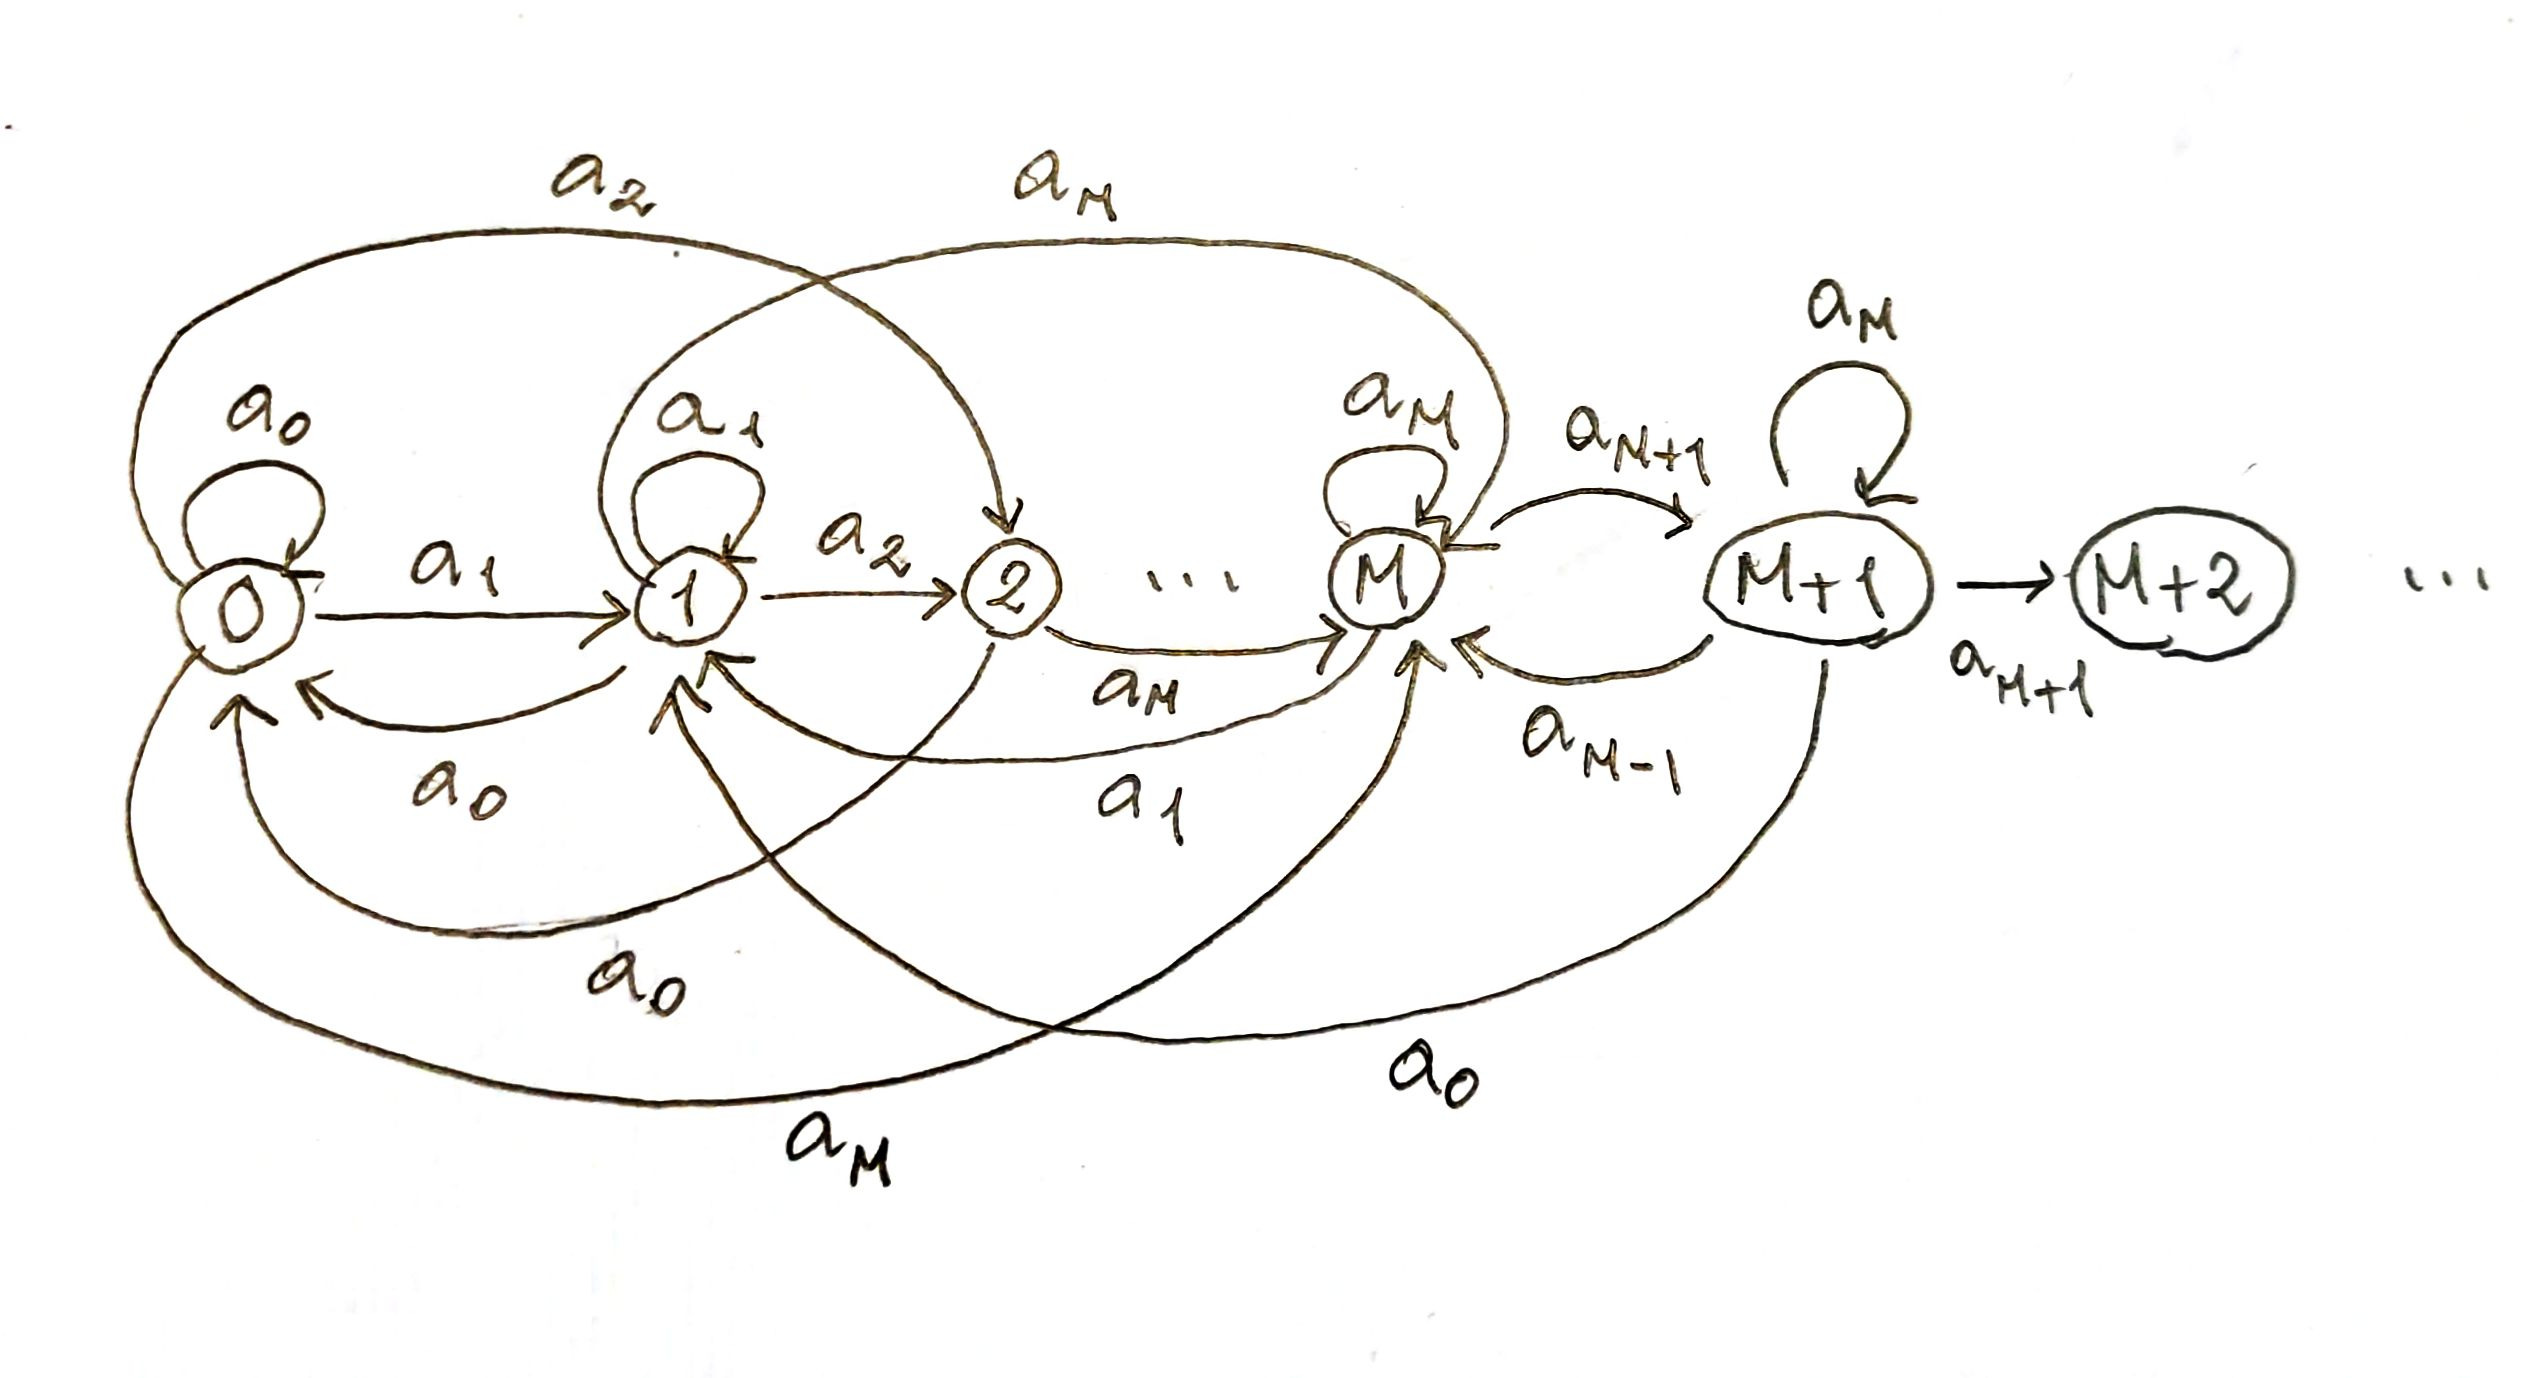
\includegraphics[width=0.7\textwidth]{block1.jpeg}
    \caption{Block diagram for protocol $1$. The transition probabilities between the first $M$ states are all the same, and \q{start to change} for the $M+1$ state onwards.\label{fig:block-diagram1}} 
\end{figure}

\subsubsection{Protocol 2}
We examine two variants: one where $M = +\infty$ (a), and one with finite $M$ (b).

For the case (2a) the evolution becomes:
\begin{align*}
    X_{n+1} = \begin{cases}
        \xi_n & X_n \geq m\\
        X_n + \xi_n & \text{otherwise}
    \end{cases}
\end{align*}
In other words, if the data is \textit{enough} ($\geq m$), we send it all (as there is no size limit), and the next state will be the one holding just the newly arrived data $\xi_n$. Otherwise, we keep all the current data $X_n$, without sending anything, and also add the newly arrived data $\xi_n$.

\medskip

The transition matrix becomes:
\begin{align*}
    P_{ij} = \begin{cases}
        a_j & X_n \geq m\\
        a_{j-1} & X_n < m
    \end{cases} \qquad \textbf{P} = \begin{blockarray}{*{7}{c} l}
        \begin{block}{l*{7}{>{\scriptstyle}c<{}}}
            & 0 & 1 & 2 & \cdots & m-2 & m-1 & \cdots \\
          \end{block}
          \begin{block}{>{\scriptstyle}r<{}(*{7}{c})}
            0 & a_0  & a_1  & a_2  & \cdots & \cdots & \cdots & \cdots \\ 
            1 & 0 & a_0 & a_1 & \cdots & \cdots & \cdots & \cdots \\ 
            \vdots & \ddots & \ddots & \ddots & \ddots & \ddots & \ddots & \vdots \\ 
            m-1 & 0 & 0 & 0 & \cdots & 0 & a_0 & \cdots \\ 
            m & a_0 & a_1 & a_2 & a_3 & \cdots & \cdots & \cdots \\ 
            m+1 & a_0 & a_1 & a_2 & a_3 & \cdots & \cdots & \cdots \\
            \vdots & \vdots & \vdots & \vdots & \vdots & \vdots & \vdots & \vdots \\
        \end{block} 
    \end{blockarray} 
\end{align*}
And the block diagram is represented in fig. \ref{fig:block2}.

\medskip

\begin{figure}[htp]
    \centering
    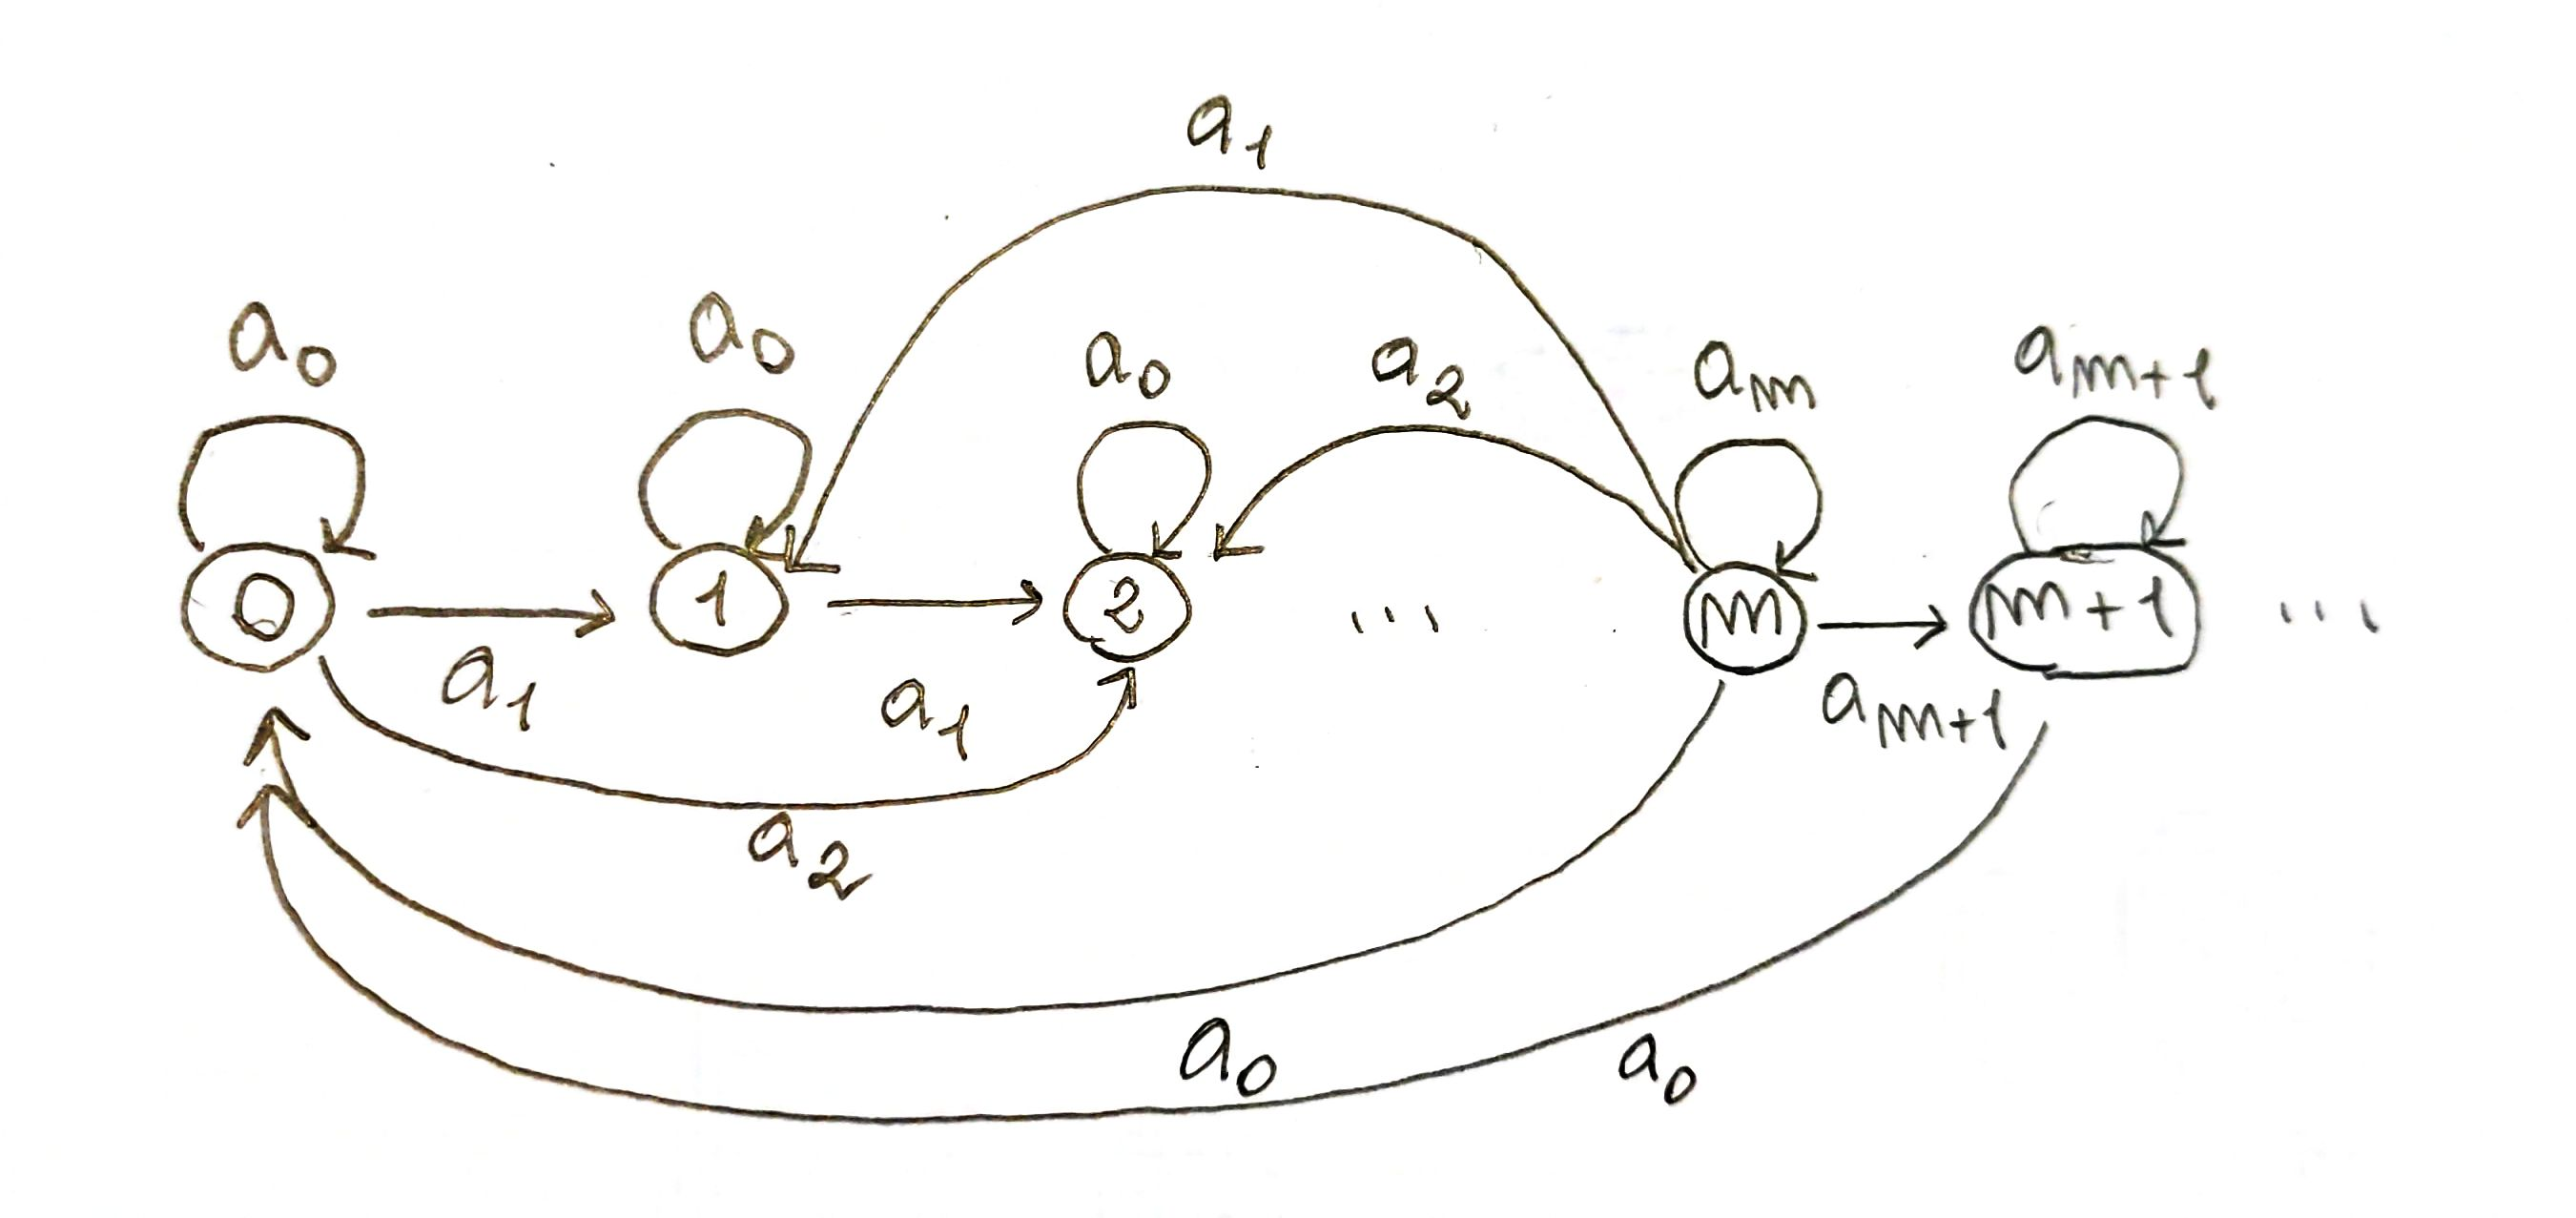
\includegraphics[width=0.7\textwidth]{block2.jpeg}
    \caption{Block diagram for protocol ($2$a), with minimum transfer size $m$ and unlimited bandwidth.\label{fig:block2}} 
\end{figure}

Finally, case (2b) is a combination of protocol 1 and (2a). The system's evolution is described by:
\begin{align*}
    X_{n+1} = \begin{cases}
        X_n + \xi_n & X_n < m\\
        \xi_n & m \leq X_n \leq M\\
        X_n - M + \xi_n & X_n > M
    \end{cases}
\end{align*}
The transition matrix becomes:
\begin{align*}
    \textbf{P} = \begin{blockarray}{*{7}{c} l}
        \begin{block}{l*{7}{>{\scriptstyle}c<{}}}
            & 0 & 1 & 2 & \cdots & m-2 & m-1 & \cdots \\
          \end{block}
          \begin{block}{>{\scriptstyle}r<{}(*{7}{c})}
            0 & a_0  & a_1  & a_2  & \cdots & \cdots & \cdots & \cdots \\ 
            1 & 0 & a_0 & a_1 & \cdots & \cdots & \cdots & \cdots \\ 
            \vdots & \ddots & \ddots & \ddots & \ddots & \ddots & \ddots & \vdots \\ 
            m-1 & 0 & 0 & 0 & \cdots & 0 & a_0 & \cdots \\ 
            m & a_0 & a_1 & a_2 & a_3 & \cdots & \cdots & \cdots \\ 
            m+1 & a_0 & a_1 & a_2 & a_3 & \cdots & \cdots & \cdots \\
            \vdots & \vdots & \vdots & \vdots & \vdots & \vdots & \vdots & \vdots \\
            M & a_0 & a_1 & a_2 & a_3 & \cdots & \cdots & \cdots\\
            M+1 & 0 & a_0 & a_1 & a_2 & \cdots & \cdots & \cdots \\
            M+2 & 0 & 0 & a_0 & a_1 & \cdots & \cdots & \cdots\\
            \vdots & \vdots & \vdots & \vdots & \vdots & \vdots & \vdots & \vdots \\
        \end{block} 
    \end{blockarray} 
\end{align*}
with the block diagram represented in fig. \ref{fig:block3}.

\begin{figure}[htp]
    \centering
    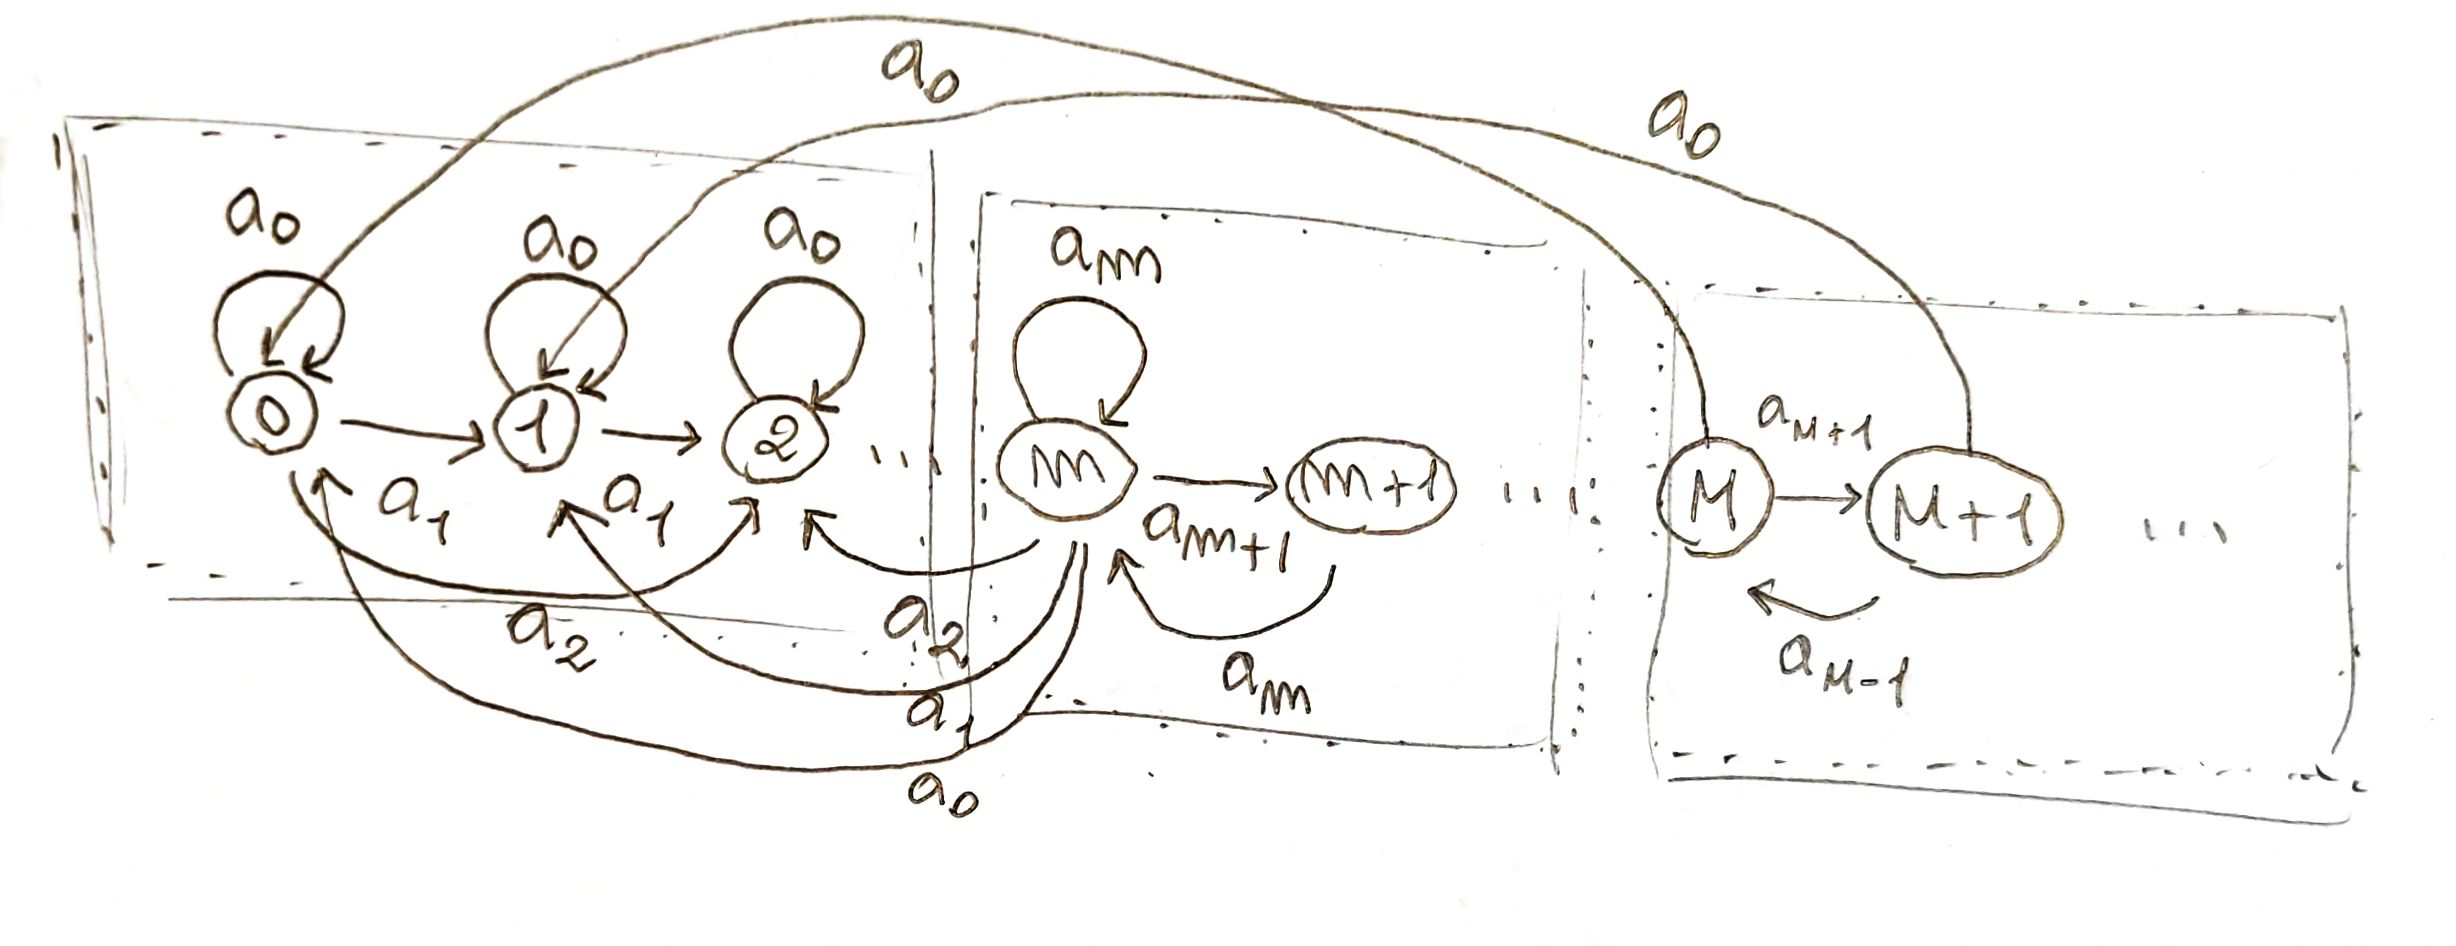
\includegraphics[width=0.7\textwidth]{block3.jpeg}
    \caption{Block diagram for protocol ($2$b), with minimum transfer size $m$ and limited bandwidth $M$.\label{fig:block3}} 
\end{figure}

Protocol 2, while more realistic than the version $1$, may lead to problem. For example, suppose that we receive too little data to send, and for many consecutive time slots we do not receive any more data. In this situation, the buffer's content will be sent after \textit{a lot of time} - and so, paradoxically, the optimization we considered to make the system more efficient now leads to a very inefficient behaviour. We can fix this by limiting the maximum number of consecutive empty slots when the queue is not empty. In other words, if we have some data ($\leq m$) in the buffer, and do not receive enough data to surpass $m$ for a certain number of time slots (e.g. $2$), we will send all the buffer's content anyway. This leads to the block diagram of fig. \ref{fig:block4}, where we \q{replicate states}, as we are keeping track of both $X_n$ and a \q{timeout counter} for sending data.

\begin{figure}[htp]
    \centering
    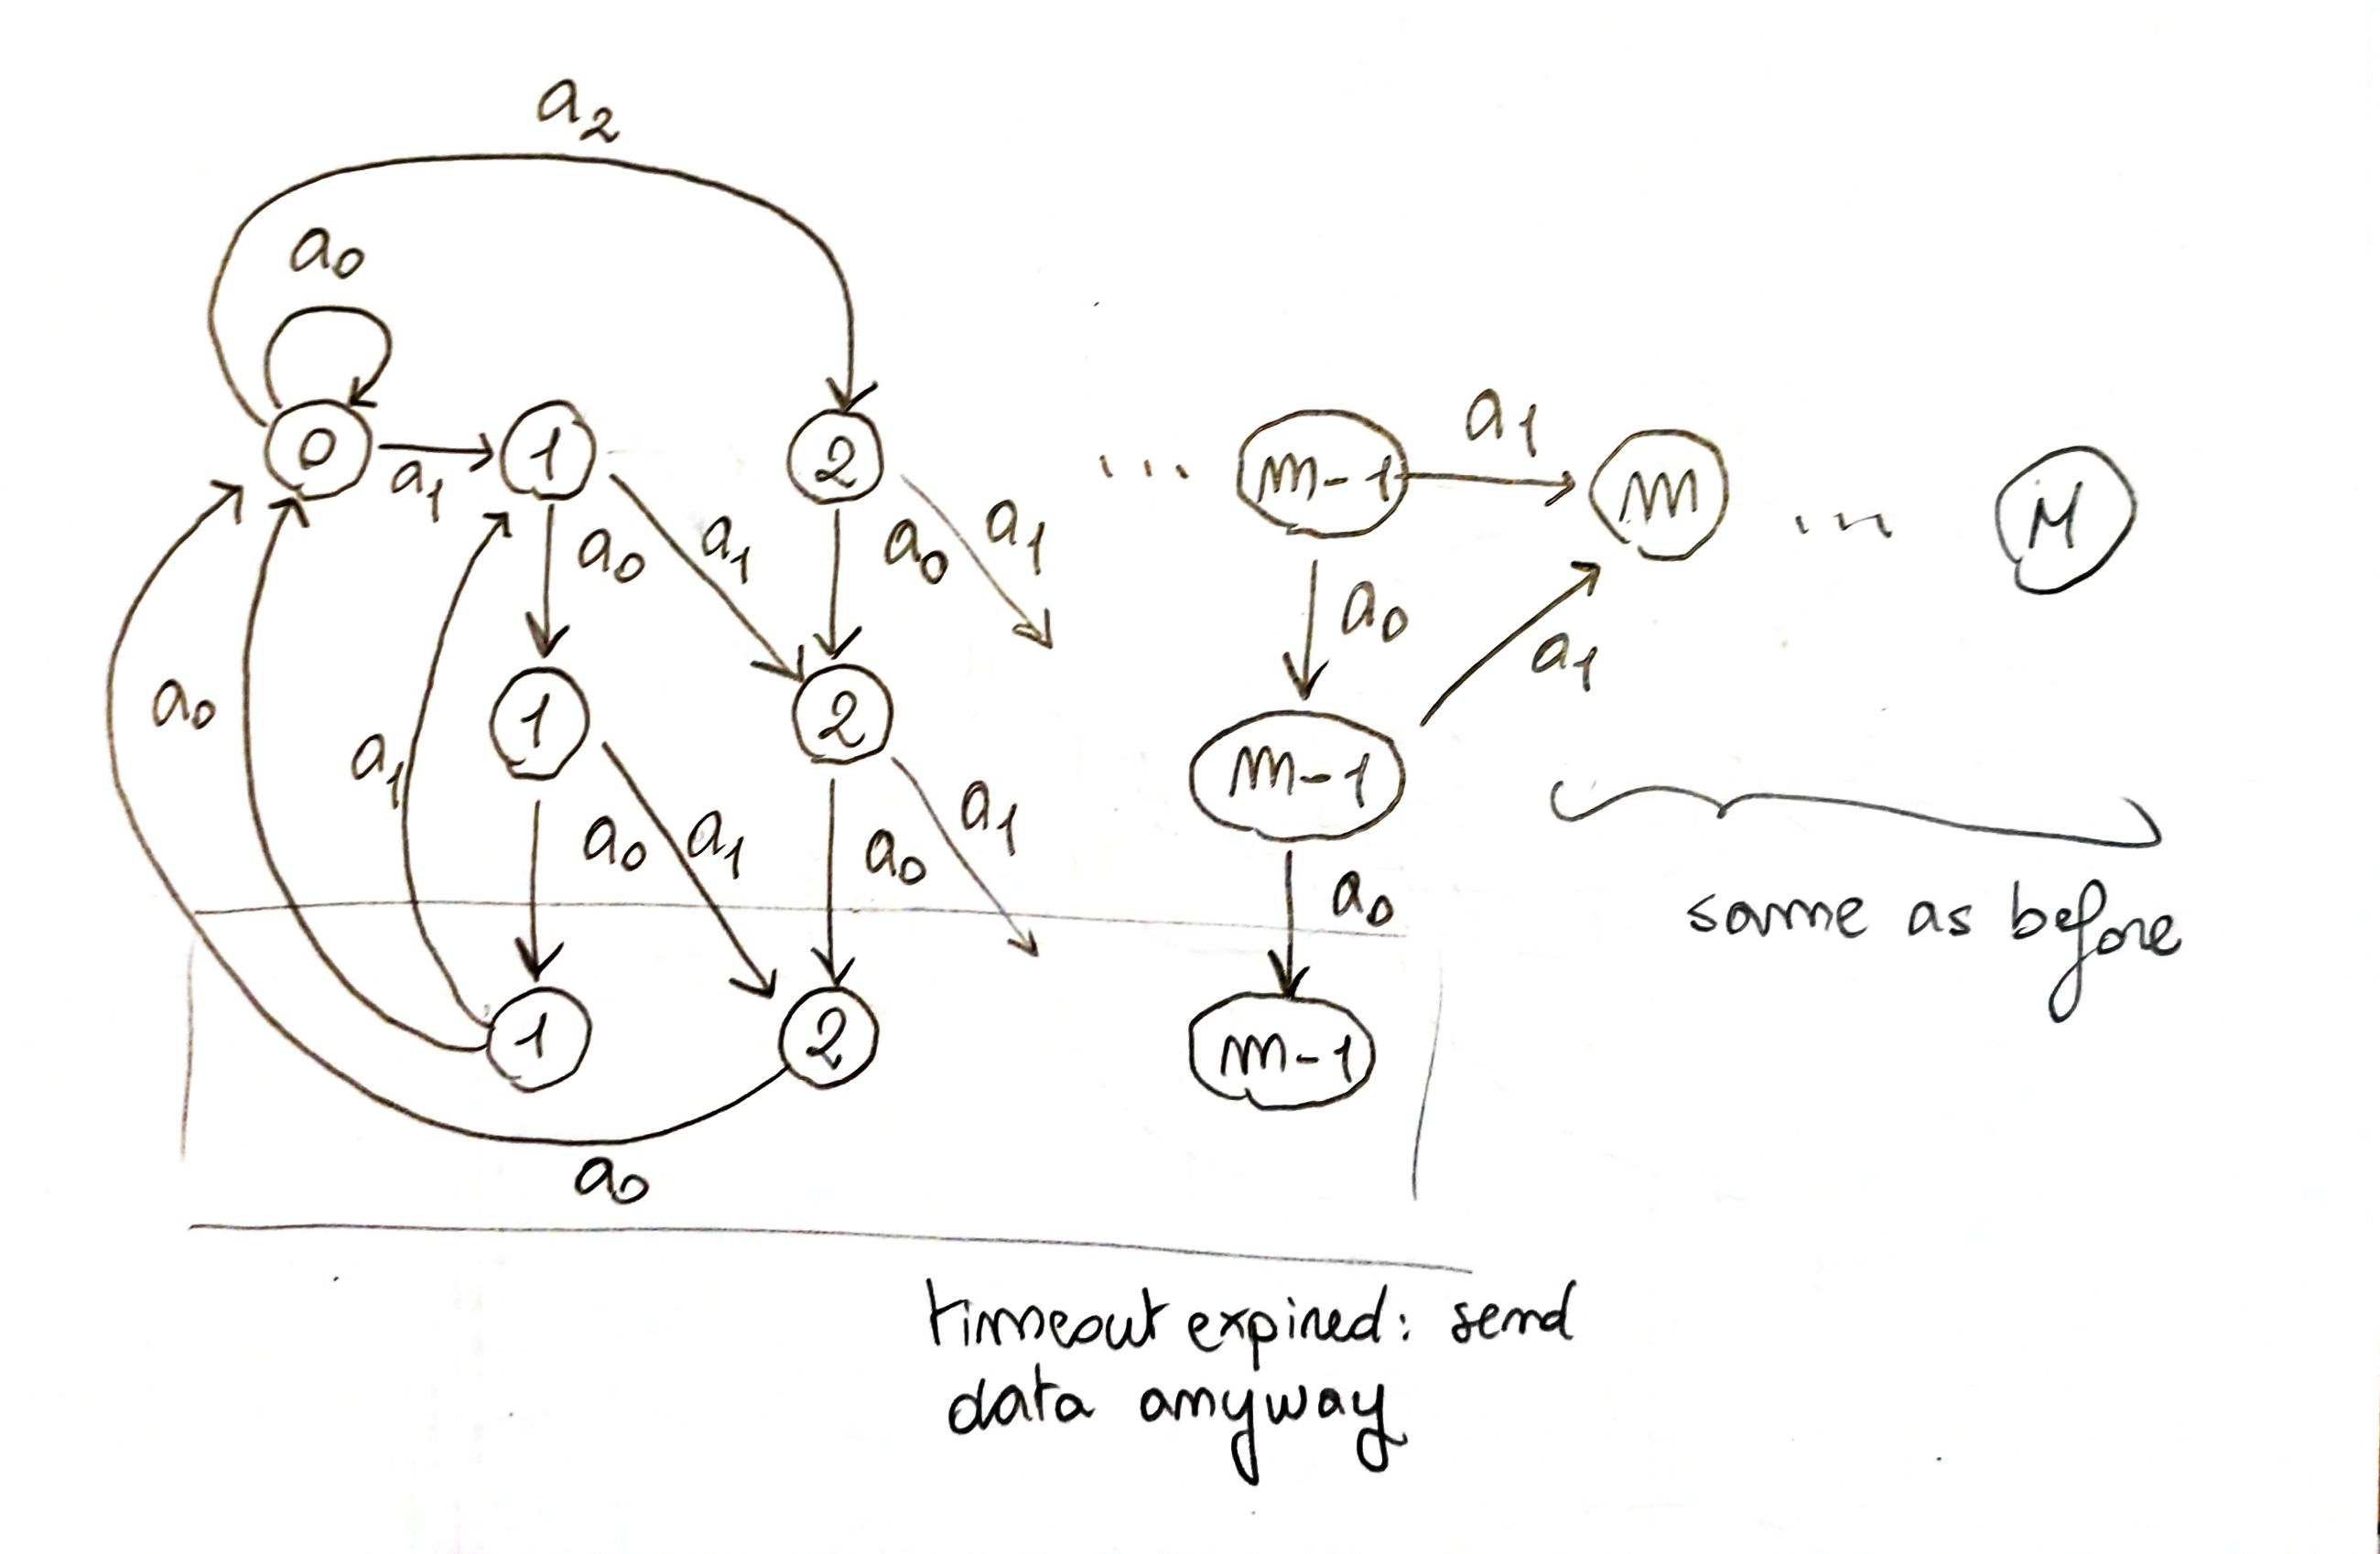
\includegraphics[width=0.7\textwidth]{block4.jpeg}
    \caption{Block diagram for protocol $2$, with minimum transfer size $m$ and a \q{timeout} for sending data of $2$ time slots. If the $m$ threshold is not reached after $2$ time slots, then the buffer's content is sent anyway.\label{fig:block4}} 
\end{figure}

\section{First step analysis}
A very useful technique for studying Markov chains is the so-called \textbf{first step analysis}, where essentially we study the probabilities \textit{conditioned} to the initial state, and write \textit{recursive relations} for the system's state.

\medskip

For example, consider the Markov chain with transition probability matrix given by:
\begin{align}\label{eqn:P-5}
    \textbf{P} = \begin{blockarray}{l*{3}{c}}
        \begin{block}{l*{3}{>{\scriptstyle}c<{}}}
            & 0 & 1 & 2\\
        \end{block}
        \begin{block}{>{\scriptstyle}r<{}(*{3}{c})}
            0 & 1 & 0 & 0\\
            1 & \alpha & \beta & \gamma \\
            2 & 0 & 0 & 1\\ 
        \end{block}
    \end{blockarray}
\end{align}
The relative block diagram is represented in fig. \ref{fig:block5}.

\begin{figure}[htp]
    \centering
    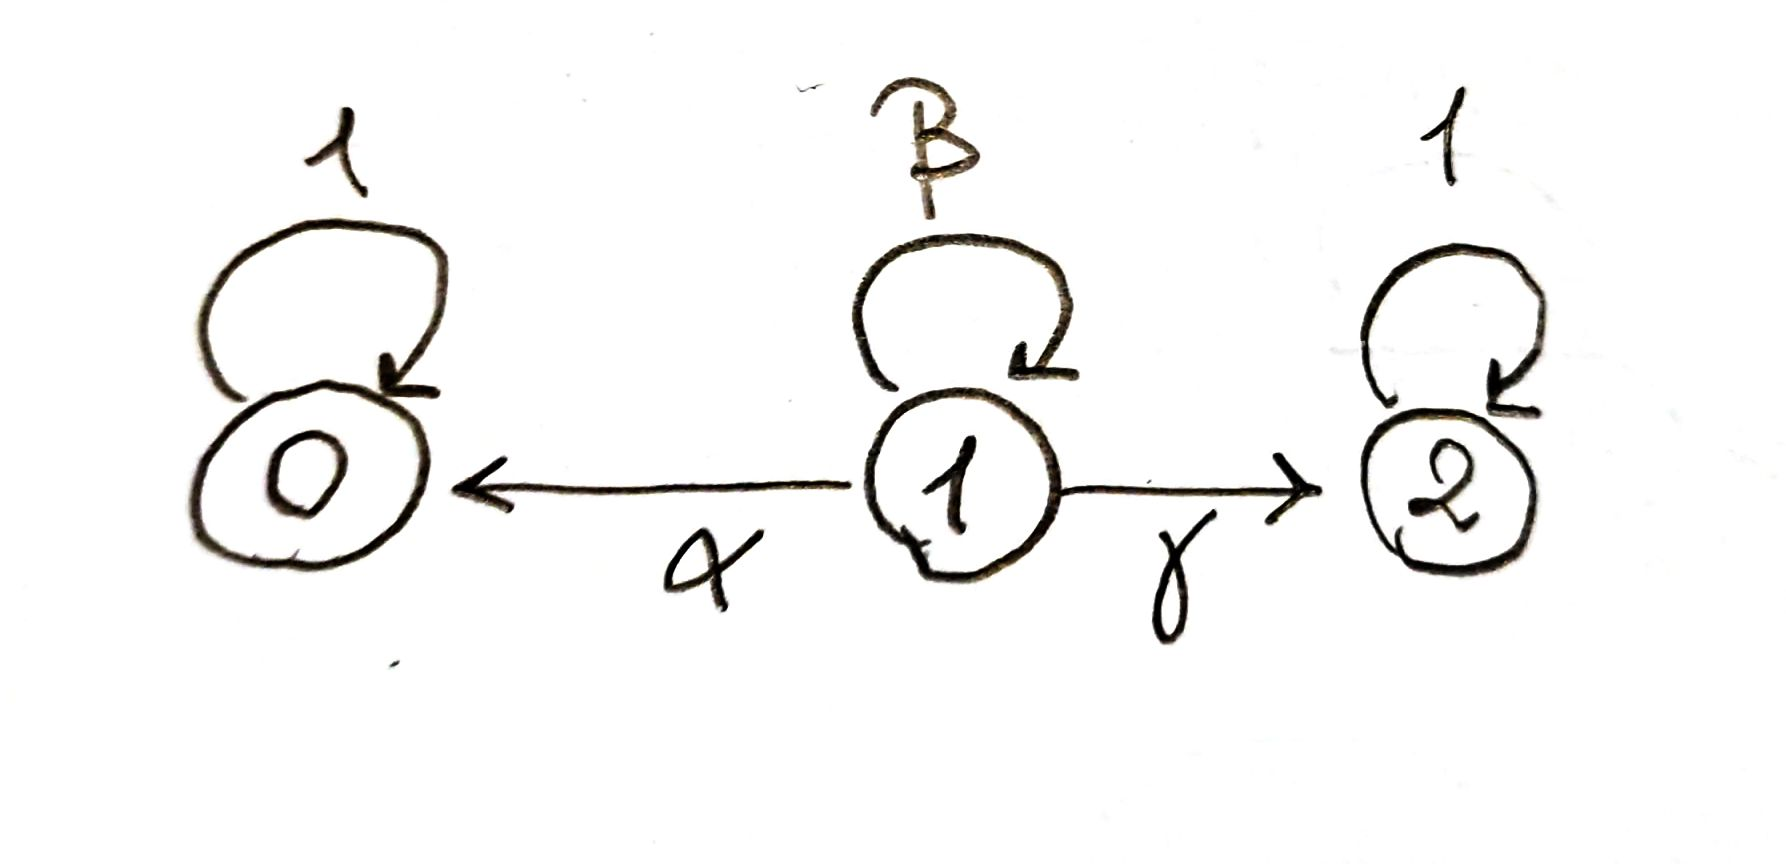
\includegraphics[width=0.7\textwidth]{block5.jpeg}
    \caption{Block diagram for the Markov chain (\ref{eqn:P-5}).\label{fig:block5}} 
\end{figure}

We note that states $0$ and $2$ do not admit transitions \textit{to}  other states, and so they are called \textbf{absorbing states}: if the system enters one of them, then it can never leave. On the other hand, state $1$ does not admit transition \textit{from} other states, and so is called a \textbf{transient state}: the system can be in state $1$ for a time, but after that it will never return there. 

\medskip

We are interested in the general behaviour of the system, and in particular:
\begin{itemize}
    \item What is the probability that the system will get \q{trapped} in either state $0$ or $2$?
    \item How long will it take to reach one of the absorbing state?
\end{itemize}

First of all, we define the \textbf{time of absorption} as the minimum number of steps (i.e. minimum \textit{time index} $n$) needed to reach one of the absorbing states:
\begin{align*}
    T \equiv \min \{n \geq 0\colon X_n \in \{0,2\}\}
\end{align*}
The absorption probability of state $0$ is given by:
\begin{align*}
    u = \mathbb{P}[X_t = 0 | X_0 = 1]
\end{align*}
(We need to start from $1$, otherwise the system would be already in an absorbing state.)

Finally, we denote with $\nu$ the average absorption time:
\begin{align*}
    \nu = \mathbb{E}[T|X_0 = 1]
\end{align*}

\medskip

In \textbf{first step analysis} we \textit{condition} the value of a parameter of interest (e.g. $u$) to the possible \textit{values} $X_1$ that the system can take after the first step. Formally, we use the law of total probability to write:
\begin{align*}
    u &= \mathbb{P}[X_t = 0 |X_0=1] = \\
    &= \sum_{k=0}^2 \mathbb{P}[X_t = 0|X_0=1, X_1 = k] \mathbb{P}[X_1 = k|X_0=1]
\shortintertext{And then apply the Markovian property to remove all conditions but the latest one:}
    &= \sum_{k=0}^2 \mathbb{P}[X_t = 0|X_1 = k] \mathbb{P}[X_1 = k | X_0 = 1]
\shortintertext{Expanding the sum and using the transition probabilities from (\ref{eqn:P-5}) we have:}
&= 1 \cdot \alpha + u \cdot \beta + 0 \cdot \gamma
\end{align*}  
We can interpret this result by \textit{imagining} all \textit{possible first steps}, starting from $X_0=1$.
\begin{itemize}
    \item From $X_0=1$ we may go to $X_1 = 0$ with probability $\alpha$. In this case we have reached $0$, and so the probability of \q{reaching $0$ after some time} is $1$ (we already did it!), meaning that $u=1$.
    \item From $X_0=1$ we could also go to $X_1=2$ with probability $\gamma$. The latter is an absorbing state, meaning that the system cannot escape it - thus reaching $0$ at a latter time is impossible, and $u=0$.
    \item In the remaining case, the system is again in $X_1=1$, with probability $\beta$. Afterwards, because of the Markovian property, the system \q{forgets} its past behaviour. So the following step will be \textit{exactly} like the first one we've just considered, and in particular the absorption probability $u$ will remain the same.
\end{itemize}
Note that now we have $u$ also in the rhs. To find it, we just rearrange:
\begin{align*}
    u = \frac{\alpha}{1-\beta}  = \frac{\alpha}{\alpha + \gamma} 
\end{align*}

\medskip

We can apply a similar reasoning to $\nu$:
\begin{align*}
    \nu &= 1 + \alpha \cdot 0 + \beta \cdot \nu + \gamma \cdot 0 =\\
    &= 1 + \beta \nu
\end{align*}
Here we need to count the first step (the absorption time must be $\geq 1$, as we are not starting in an absorbing state). With probability $\alpha$ and $\gamma$ the system moves to an absorbing state, meaning that no more steps are required to reach them. However, with probability $\beta$ the system remains in $1$, where the expected absorption time is still $\nu$. Rearranging:
\begin{align*}
    \nu = \frac{1}{1-\beta} 
\end{align*}

We can check this by noting that the amount of time spent in state $1$ has a geometric distribution. Then, as every transition to other states from $1$ leads to an absorbing states, meaning that the absorption time is exactly the time \q{spent} by the system in state $1$, we have:
\begin{align*}
    \mathbb{P}[T > k|X_0 = 1] = \beta^k \Rightarrow \mathbb{E}[T|X_0 = 1] = \sum_{k=0}^{+\infty} \mathbb{P}[T>k|X_0=1] = \frac{1}{1-\beta} 
\end{align*}
However, this direct computation will be impossible in more complex case, while the first-step approach will still remain feasible.

\medskip

For example, consider the slightly more complex case of a $4$-state system:
\begin{align}\label{eqn:P-6}
    \textbf{P} = \begin{blockarray}{l*{4}{c}}
        \begin{block}{l*{4}{>{\scriptstyle}c<{}}}
            & 0 & 1 & 2 & 3\\
        \end{block}
        \begin{block}{>{\scriptstyle}r<{}(*{4}{c})}
            0 & 1 & 0 & 0 & 0\\
            1 & P_{10} & P_{11} & P_{12} & P_{13}\\
            2 & P_{20} & P_{21} & P_{22} & P_{23}\\
            3 & 0 & 0 & 0 & 1 \\
        \end{block}
    \end{blockarray}
\end{align}

\begin{figure}[htp]
    \centering
    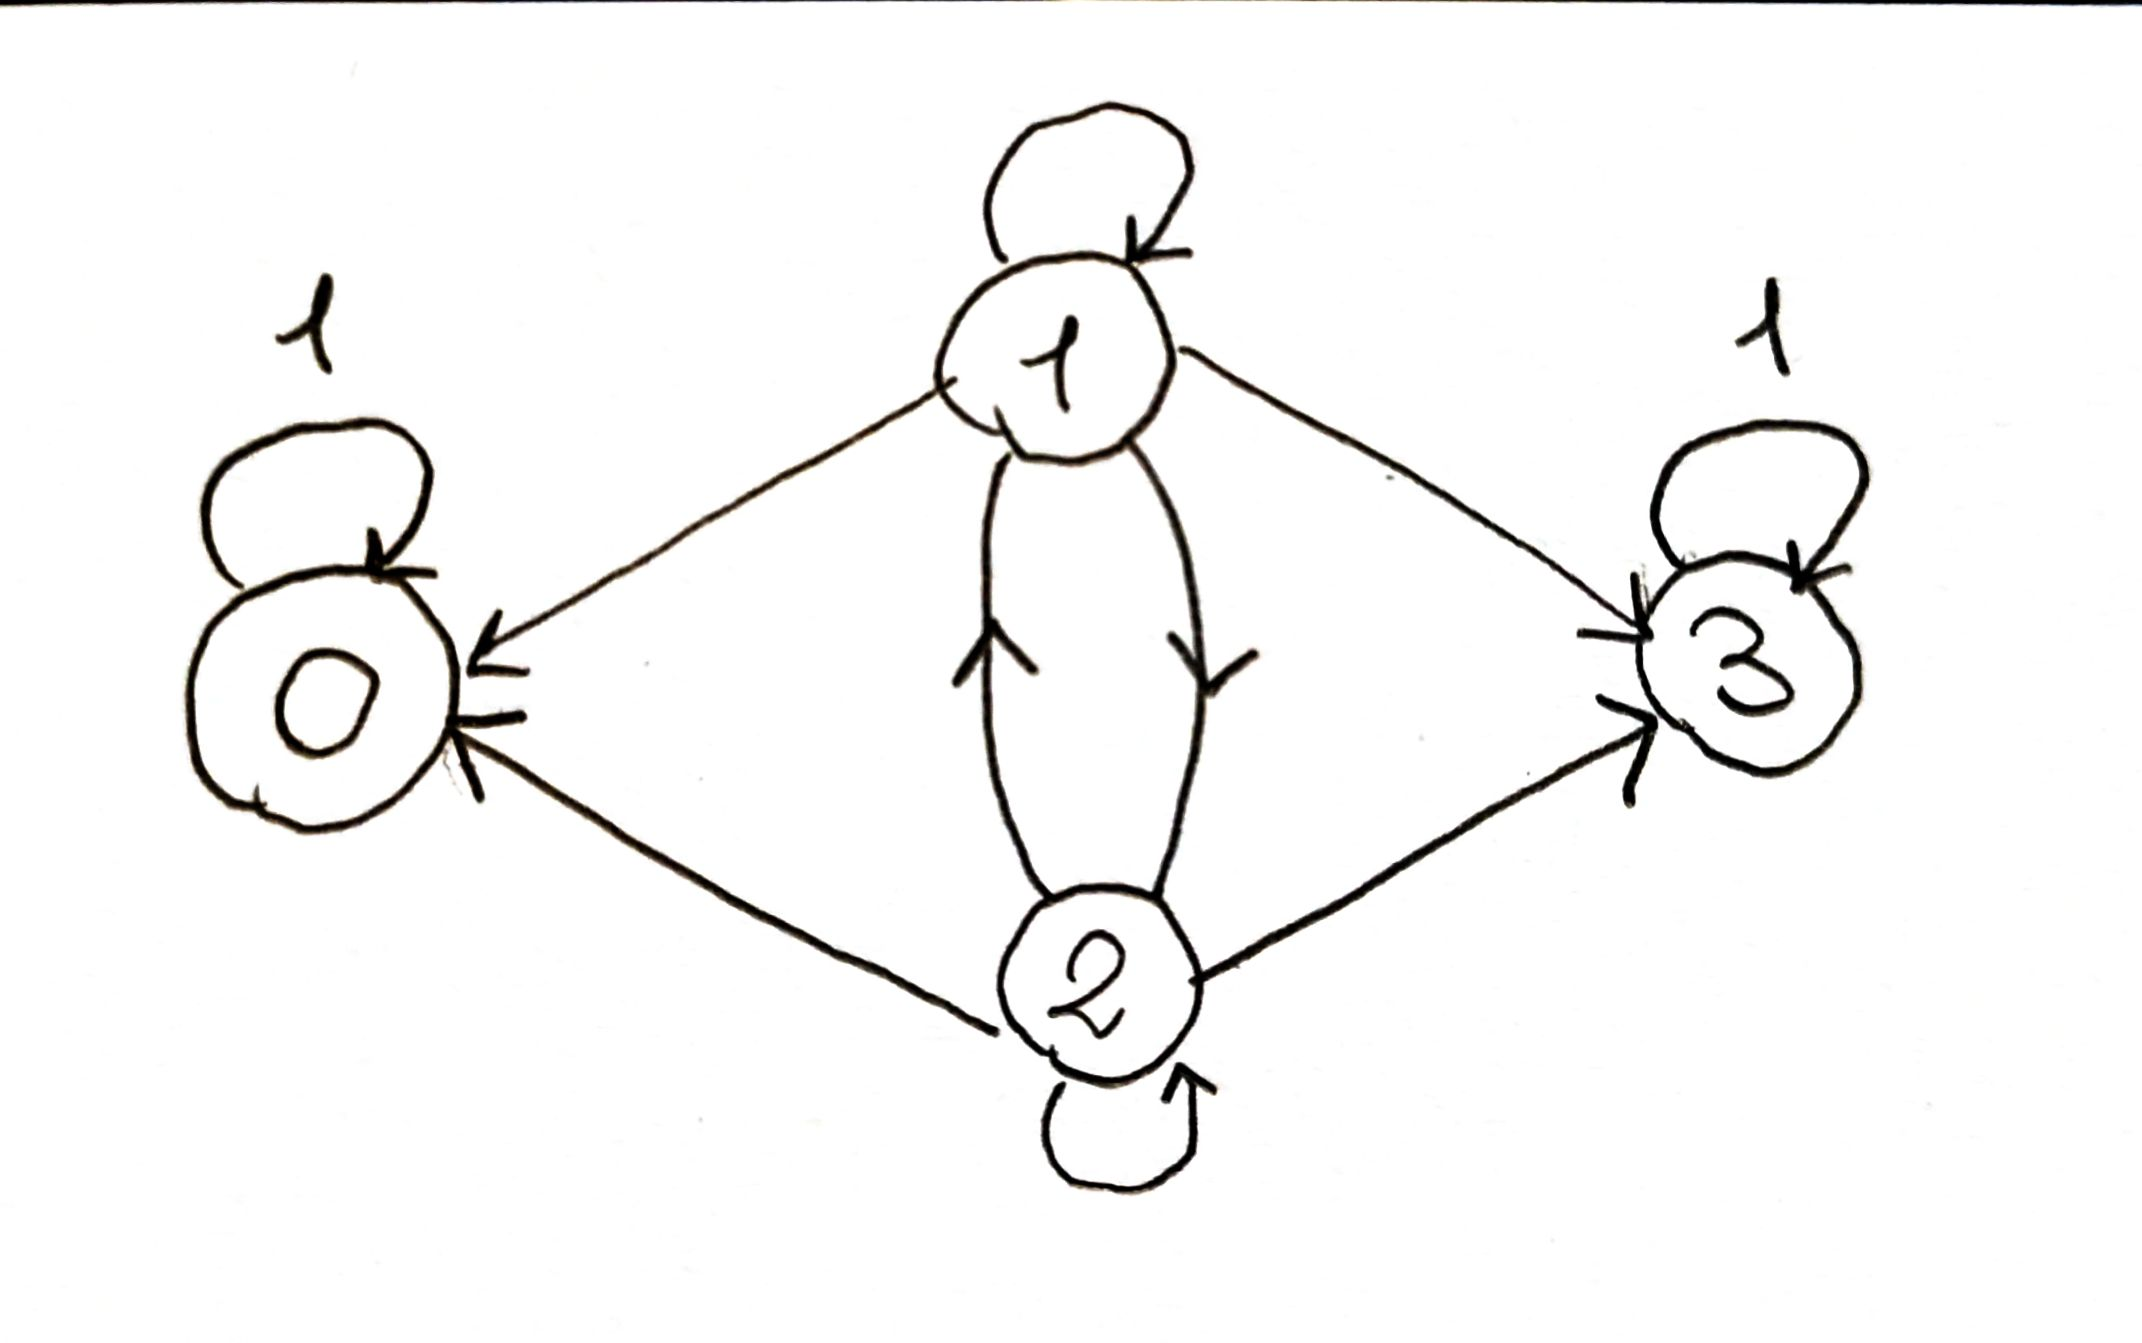
\includegraphics[width=0.7\textwidth]{block6.jpeg}
    \caption{Block diagram for the Markov chain (\ref{eqn:P-6}).\label{fig:block6}} 
\end{figure}

As before, we define the absorption time as the minimum time index needed to reach an absorbing state:
\begin{align*}
    T = \min \{n \geq 0\colon X_n \in \{0,3\}\}
\end{align*}
We now have two possible initial states, and thus two absorption probabilities (concerning the final state $0$):
\begin{align*}
    u_i = \mathbb{P}[X_t = 0|X_0=i] \qquad i=1,2
\end{align*}
And two averages:
\begin{align*}
    \nu_i = \mathbb{E}[T|X_0=i] \qquad i=1,2
\end{align*}

First-step analysis applied to the initial state $1$ leads to:
\begin{align}\label{eqn:u1}
    u_1 = 1 \cdot P_{10} + 0 \cdot P_{13} + u_1 \cdot P_{11} + u_2 \cdot P_{12}
\end{align}
Similarly, for initial state $2$ we have:
\begin{align}\label{eqn:u2}
    u_2 = 1 \cdot P_{20} + 0 \cdot P_{23} + u_1 \cdot P_{21} + u_2 \cdot P_{22}
\end{align}
Equations (\ref{eqn:u1}) and (\ref{eqn:u2}) can then be solved to find $u_1$ and $u_2$.

\medskip

The same reasoning can be applied to $\nu_i$:
\begin{align*}
    \nu_1 &= 1 + 0 \cdot (P_{10} + P_{13}) + \nu_1 \cdot P_{11} + \nu_2 \cdot P_{12}\\
    \nu_2 &= 1 + 0 \cdot (P_{20} + P_{23}) + \nu_1 \cdot P_{21} + \nu_2 \cdot P_{22}
\end{align*}

\medskip

In a more \textbf{general case}, we will have a number of states $0, 1, \dots, N$. Suppose that $0,1,\dots, r-1$ are \textbf{transient} states, and $r,\dots,N$ are \textbf{absorbing}. The transition matrix has the form:
\begin{align}\label{eqn:P-7}
    \textbf{P} = \begin{blockarray}{l*{2}{c}}
        \begin{block}{l*{2}{>{\scriptstyle}c<{}}}
            & 0\cdots N-r+1 & N-r\cdots N \\
        \end{block}
        \begin{block}{>{\scriptstyle}r<{}(*{2}{c})}
            0\cdots N-r+1 & \textbf{Q}  & \textbf{R} \\
            N-r\cdots N & \textbf{0}   & \mathbb{I}\\
        \end{block}
    \end{blockarray}
\end{align}
In fact the last $N-r$ states have a \textit{certain} transition probability only to themselves, and so their rows have $0$\textit{s} for the first $r$ entries, and exactly a single $1$ in the rest. The \textbf{Q} block regulates transition between transient states, while the \textbf{R} block the ones between transients and absorbing.  

\medskip

As in general there are more than $2$ absorbing states, we need to specify \textit{which one we are considering} for the absorption probabilities:
\begin{align*}
    u_i \equiv U_{ik} &= \mathbb{P}[\text{Absorption in $k$}|X_0 = i] = \qquad (0\leq i < r)\\
    &= \sum_{j=0}^N \mathbb{P}[\text{Absorption in $k$}|X_0=i, X_1 = j]P_{ij} =\\
    &= \underbrace{P_{ik}\cdot 1 }_{\parbox{5em}{\footnotesize \centering Abs. state we are considering}}+ \underbrace{\sum_{\substack{j = r\\j \neq k}}^N P_{ij} \cdot 0 }_{\parbox{5em}{\footnotesize\centering Other abs. states}}+ \underbrace{\sum_{j=0}^{r-1} P_{ij} \cdot u_j}_{\parbox{5em}{\centering\footnotesize Transient states}} =\\
    &= P_{ik} + \sum_{j=0}^{r-1} P_{ij} U_{jk} \qquad i=0,1,\dots, r-1
\end{align*} 

\end{document}
